\documentclass{beamer}
\usepackage[utf8]{inputenc}
\usepackage[english]{babel} % Adds processing for some simple special characters.

% Packages for better page formatting and nice footnotes. %

\usepackage{fancyhdr} % Headers.
\usepackage{multicol} % Columns.

\renewcommand{\thefootnote}{\fnsymbol{footnote}}

% Utilities for fine-grained control over image insertion. %

\usepackage{graphicx} % Insert images.
\usepackage{float} % Images float in document environment.
\usepackage{wrapfig} % Image/tables in multicols with \wrapfigure or \wraptable.
\usepackage[justification=centering]{caption} % Captions for single images.
\usepackage{subcaption} % Captions for simultaneous images.
\graphicspath{{./img/}}

% Some utilities for scientific and mathematical writing. %

\usepackage{siunitx} % Formatting for numbers with SI units.
\usepackage{amsmath} % Astronomical symbols.
\usepackage{isotope} % Nice markup syntax for chemical symbols.
\usepackage{xfrac}   % Slant fractions and other utilities.
\usepackage{lipsum}  % Generate pseudo-text for formatting.
\usepackage{listings}

% Utilities for manual kerning adjustment. %

\newcommand\K{\kern.05em} % Small amount of kerning.
\newcommand\KK{\kern.1em} % Medium amount of kerning.
\newcommand\KKK{\kern.2em} % Large amount of kerning.
\newcommand\KKKK{\kern.3em} % Very large amount of kerning.

% Utilities for Beamer slides. %

\usecolortheme{mit}
\usepackage{epstopdf}
\setbeamertemplate{navigation symbols}{}

% Bibliography and referencing style.

\usepackage[backend=bibtex,style=phys,sorting=nyt]{biblatex} % Use style=draft for troubleshooting.
\addbibresource{references.bib}

% Title and author for title page. %

\title{Bayesian Inference of Star Formation History in the Host Galaxies of Tidal Disruption Events}
\author{Alexander S. Wheaton \\ Supervisor: Andy Lawrence, FRSE}
\institute[UoE]{
\includegraphics[width=0.3\textwidth]{crest}\vspace{1em}}
\date{\today}

\begin{document}

\begin{frame}
  \titlepage
\end{frame}

\begin{frame}{Project Aims}
  \begin{figure}[L]
    \includegraphics[width=\textwidth]{AT2019qiz_host_red}
    % \includegraphics[width=\textwidth]{iPTF16fnl_host_red}
    % \includegraphics[width=\textwidth]{ASASSN-14li_host_red}
    \caption{AT2019qiz Host Galaxy}
  \end{figure}
  \begin{itemize}
    \item Investigate the statistical behaviour of the star formation in the host galaxies of tidal disruption events.
  \end{itemize}
\end{frame}

\begin{frame}{Motivation: XSHOOTER Targets}
  \begin{table}
    \begin{tabular}{| l | c | r |}
      \hline
      TDE         & $m$ & z        \\
      \hline
      ASASSN-14li & 15  & 0.0206   \\
      ASASSN-15oi & 16  & 0.0484   \\
      AT2018fyk   & 17  & 0.06     \\
      AT2019ahk   & 17  & 0.026211 \\
      AT2019azh   & 15  & 0.022    \\
      AT2019dsg   & 15  & 0.0512   \\
      AT2019qiz   & 15  & 0.01513  \\
      iPTF16fnl   & 16  & 0.018    \\
      AT2018hyz   & 17  & 0.04573  \\
      ASASSN-14ae & 17  & 0.0436   \\
      \hline
    \end{tabular}
    \caption{The XSHOOTER targets on tidal disruption events.}
  \end{table}
\end{frame}

\begin{frame}{Active Galactic Nuclei (AGN)}
  \section{Key Features}
  \begin{itemize}
    \item Compact, highly luminous nuclear region.
    % From 10^35 W to 10^42 W, Milky Way core is 10^10 W.
    \item Broad spectral energy distribution.
    % Non-stellar emission which is inexplicable by blackbody radiation.
    \item Strong (and sometimes broad) emission lines.
    % Which if due only to the Doppler effect, imply gas motions of $v = 10000 km/s$.
    \item Variability over short timescales.
    % Minutes to days, in some cases a few years.
    % \item Upper bound on size $\approx 100 pc$ \cite{Peterson_1997} % Determined by spatial resolution, but requires 10% galactic mass to be central
    % \item For smaller $r$, need extraordinary energy production.\cite{Peterson_1997}
  \end{itemize}
\end{frame}

\begin{frame}{Active Galactic Nuclei (AGN)}
  \begin{figure}
    \centering
    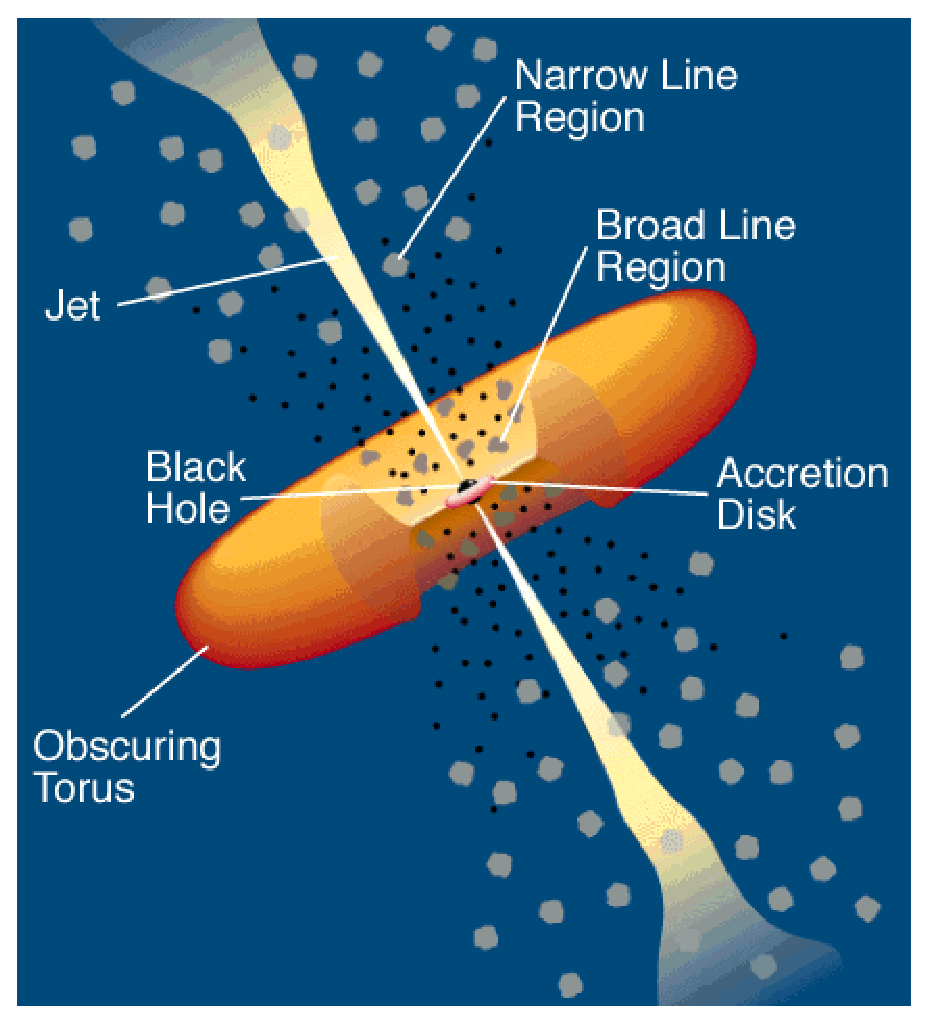
\includegraphics[width=0.5\textwidth]{agn_model}
    \caption{Accretion of matter onto surface of a black hole. Image adapted from Urry and Padovani 1995.}
  \end{figure}
\end{frame}

\begin{frame}{The Starburst-AGN Connection}
  \begin{figure}
    \centering
    \includegraphics[width=0.5\textwidth]{image--002}
    \caption{Strong relationship between star formation and black hole mass. Image adapted from Veilleux 2008.}
  \end{figure}

  \begin{itemize}
    \item Cosmologically important impact on galaxy formation and evolution.
  \end{itemize}
\end{frame}

\begin{frame}{Possible mechanisms?}
  \begin{itemize}
    \item Gas or radiation pressure from starbursts and/or AGN-driven wind shuts off  black hole fuel supply.
    \item Direction of causation unclear.
    \item AGN is a possible source of quenching.
    \item Need more information...
  \end{itemize}
\end{frame}

\begin{frame}{Tidal Disruption Events}
  \begin{figure}
    \includegraphics[width=0.75\textwidth]{tidal_disruption_event}
    \caption{TDE impression, image credit NASA/JPL-Caltech.}
    % https://images.nasa.gov/details-PIA20027
    \label{img:tde_impression}
  \end{figure}
  \begin{itemize}
    \item Do TDEs exhibit the same statistical behaviour?
  \end{itemize}
\end{frame}


\begin{frame}{The BAGPIPEs Module}
  \textbf{Bayesian Analysis of Galaxies for Physical Inference and Parameter EStimation.}
  \vspace{0.5in}
  \begin{itemize}
    \item Simulation of galactic spectra from SFH.
    \item Fit real spectra to plausible SFH.
  \end{itemize}
\end{frame}

\begin{frame}{The BAGPIPEs Module}
  \begin{figure}
    \centering
    \includegraphics[width=0.9\textwidth]{model020_sfh}
    \includegraphics[width=\textwidth]{model020_spectrum}
    \caption{Simulated SFH and spectrum.}
  \end{figure}
\end{frame}

\begin{frame}{The BAGPIPEs Module}
  \begin{figure}
    \centering
    \includegraphics[width=0.9\textwidth]{host_hyz_specwerr_fit}
    \includegraphics[width=0.9\textwidth]{host_hyz_specwerr_sfh}
    \caption{Observed and fitted spectrum, with inferred SFH.}
  \end{figure}
\end{frame}

\begin{frame}{Stellar Population Dating}
  \begin{figure}
    \centering
    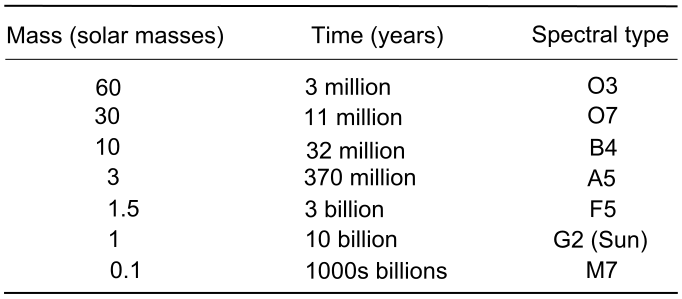
\includegraphics[width=0.9\textwidth]{lifetimes}
    \caption{Stellar lifetimes and spectral type.}
  \end{figure}
  \begin{itemize}
    \item Poor temporal resolution in SFR beyond 1 billion years.
  \end{itemize}
\end{frame}

\begin{frame}{Stellar Population Dating}
  \begin{figure}
    \centering
    \includegraphics[width=0.9\textwidth]{Screenshot}
    \caption{Number density of spectral types. Table adapted from Glenn 2001.}
  \end{figure}
  \begin{itemize}
    \item Poor temporal resolution beyond ~1 billion years.
  \end{itemize}
\end{frame}

\begin{frame}{Stellar Population Dating}
  \begin{itemize}
    \item Solution? Parameterise metallicity as well.
    \item How do Lyman and Balmer series lines evolve with starburst age?
    \item What about other metal lines?
  \end{itemize}
\end{frame}

\begin{frame}{}
  \begin{figure}
    \centering
    \includegraphics[width=\textwidth]{figure}
    \caption{Variance in flux, over starburst evolved from z=2.2 to z=0.01.}
  \end{figure}
\end{frame}

\begin{frame}{}
  \begin{figure}
    \centering
    \includegraphics[width=\textwidth]{figure1}
    \caption{Deltas in flux, over starburst evolved from z=2.2 to z=0.01.}
  \end{figure}
\end{frame}

\begin{frame}{SFH Inference - What is possible?}
  \begin{itemize}
    \item Blind fitting of spectra with known priors.
    \item Fitting multiple SFH forms.
    \item Iterative fitting.
  \end{itemize}
\end{frame}

\begin{frame}{Exploring the SFH Parameter Space}
  \textbf{R1: Entire Parameter Space with Two Components}
  \begin{figure}
    \centering
    \includegraphics[width=\textwidth]{../pipes/plots/r0_priors/phil_model_4_sfh}
    \caption{Example SFH.}
  \end{figure}
  \begin{itemize}
    \item Constrain z to be less than or equal to the TDE targets
    \item Assume separate bulk formation and burst events
  \end{itemize}
  % Assume most of stellar mass formed in a separate event
  % Let burst vary over entire history of the universe
  % Brief discussion of cosmic noon, with contrast between spirals and ellipticals
\end{frame}

\begin{frame}{Exploring the SFH Parameter Space}
  \textbf{R2 \& R3: Iterative Fitting}
  \begin{figure}
    \centering
    \includegraphics[width=\textwidth]{../pipes/plots/r0_priors/phil_model_4_sfh}
    \caption{Example SFH.}
  \end{figure}
  \begin{itemize}
    \item Insist burst component is younger than the bulk formation
  \end{itemize}
\end{frame}

\begin{frame}{Exploring the SFH Parameter Space}
  \begin{figure}
    \centering
    \includegraphics[width=0.75\textwidth]{../pipes/plots/r0_priors/phil_model_4_sfh}
    \includegraphics[width=0.75\textwidth]{../pipes/plots/r2_delayed_burst_wide/phil_model_4_sfh}
    \caption{Prior and posterior SFH.}
  \end{figure}
  \begin{itemize}
    \item ``Best''fits favour single component star formation.
  \end{itemize}
\end{frame}

\begin{frame}{Selecting Physically Reasonable Priors}
  \begin{figure}
    \centering
    \includegraphics[width=\textwidth]{../pipes/plots/r0_priors/phil_model_4_sfh}
    \caption{Example SFH.}
  \end{figure}
  \begin{itemize}
    \item SPS limits burst detection.
    \item Precise form of old formation is unimportant.
  \end{itemize}
  % SPS limits burst detection to ages <3Gyr
  % Precise form of old formation is unimportant
  % Temporal resolution is poor beyond A type stars
\end{frame}

\begin{frame}{Selecting Physically Reasonable Priors}
  \textbf{R4: Fixed Old Component, Free Burst Component}
  \begin{figure}
    \centering
    \includegraphics[width=\textwidth]{../pipes/plots/r0_priors/phil_model_4_sfh}
    \caption{Example SFH.}
  \end{figure}
  \textbf{Conclusion:}
  \begin{itemize}
    \item Impose a lower limit on bulk formation age and mass.
    \item Impose an upper limit on burst age, but let mass vary freely.
  \end{itemize}
\end{frame}

\begin{frame}{Selecting Physically Reasonable Priors}
  \textbf{R4: Fixed Old Component, Free Burst Component} \\
  \vspace{0.5in}
  \textbf{Other refined priors:}
  \begin{center}
    \begin{itemize}
      \item Velocity dispersion, $\sigma_v$
      \item Birth cloud lifetime, $\tau_{BC}$
      \item Metallicity, $Z$
      \item Extinction, $A_V$
      \item Nebular ionisation, $U$
    \end{itemize}
  \end{center}
  % Decay times/slopes of functional forms
  % Want to be consistent with Hubble morphology & redshifts of TDE data
\end{frame}

\begin{frame}{Blind Fitting Results with R4 Priors}
  \begin{figure}
    \centering
    \includegraphics[width=0.75\textwidth]{../pipes/plots/r0_priors/phil_model_8_sfh}
    \includegraphics[width=0.75\textwidth]{../pipes/plots/r4_dblplaw_burst/phil_model_8_sfh}
    \caption{Prior and posterior SFH.}
  \end{figure}
\end{frame}

\begin{frame}{Blind Fitting Results with R4 Priors}
  \begin{figure}
    \centering
    \includegraphics[width=0.75\textwidth]{../pipes/plots/r0_priors/phil_model_9_sfh}
    \includegraphics[width=0.75\textwidth]{../pipes/plots/r4_lognormal_burst/phil_model_9_sfh}
    \caption{Prior and posterior SFH.}
  \end{figure}
\end{frame}

\begin{frame}{Blind Fitting Results with R4 Priors}
  \begin{figure}
    \centering
    \includegraphics[width=0.75\textwidth]{../pipes/plots/r0_priors/phil_model_2_sfh}
    \includegraphics[width=0.75\textwidth]{../pipes/plots/r4_delayed_burst/phil_model_2_sfh}
    \caption{Prior and posterior SFH.}
  \end{figure}
\end{frame}

\begin{frame}{Blind Fitting Results with R4 Priors}
  \begin{figure}
    \centering
    \includegraphics[width=0.75\textwidth]{../pipes/plots/r0_priors/phil_model_5_sfh}
    \includegraphics[width=0.75\textwidth]{../pipes/plots/r4_delayed_burst/phil_model_5_sfh}
    \caption{Prior and posterior SFH.}
  \end{figure}
\end{frame}

\begin{frame}{Blind Fitting Results with R4 Priors}
  \begin{figure}
    \centering
    \includegraphics[width=0.75\textwidth]{../pipes/plots/r0_priors/phil_model_4_sfh}
    \includegraphics[width=0.75\textwidth]{../pipes/plots/r4_dblplaw_burst/phil_model_4_sfh}
    \caption{Prior and posterior SFH.}
  \end{figure}
\end{frame}

\begin{frame}{Correlated Parameters}
  \begin{figure}
    \centering
    \includegraphics[width=0.75\textwidth]{../pipes/plots/r4_exponential_burst/phil_model_4_corner}
    \caption{Correlation between decay time and burst mass.}
  \end{figure}
\end{frame}

\begin{frame}{Application to XSHOOTER Data}
  \begin{figure}
    \centering
    \includegraphics[width=\textwidth]{../pipes/plots/r4_dblplaw_burst/AT2019ahk_sfh}
    \caption{Posterior SFH for AT2019ahk.}
  \end{figure}
\end{frame}

\begin{frame}{Application to XSHOOTER Data}
  \begin{figure}
    \centering
    \includegraphics[width=\textwidth]{../pipes/plots/r4_dblplaw_burst/AT2019azh_sfh}
    \caption{Posterior SFH for AT2019azh.}
  \end{figure}
\end{frame}

\begin{frame}{Application to XSHOOTER Data}
  \begin{figure}
    \centering
    \includegraphics[width=\textwidth]{../pipes/plots/r4_delayed_burst/iPTF16fnl_sfh}
    \caption{Posterior SFH for iPTF16fnl.}
  \end{figure}
\end{frame}

\begin{frame}{Application to XSHOOTER Data}
  \begin{figure}
    \centering
    \includegraphics[width=\textwidth]{../pipes/plots/r4_exponential_burst/ASASSN14li_sfh}
    \caption{Posterior SFH for ASASSN14li.}
  \end{figure}
\end{frame}

\begin{frame}{Application to XSHOOTER Data}
  \begin{figure}
    \centering
    \includegraphics[width=\textwidth]{../pipes/plots/r4_exponential_burst/ASASSN15oi_sfh}
    \caption{Posterior SFH for ASASSN15oi.}
  \end{figure}
\end{frame}

\begin{frame}{Application to XSHOOTER Data}
  \begin{figure}
    \centering
    \includegraphics[width=\textwidth]{../pipes/plots/r4_lognormal_burst/AT2019dsg_sfh}
    \caption{Posterior SFH for AT2019dsg.}
  \end{figure}
\end{frame}

\begin{frame}{Conclusions}
  \begin{figure}
    \includegraphics[width=0.75\textwidth]{tidal_disruption_event}
    \caption{TDE impression, image credit NASA/JPL-Caltech.}
    % https://images.nasa.gov/details-PIA20027
    \label{img:tde_impression}
  \end{figure}
  \begin{itemize}
    \item Starbusts are detectable \textbf{IF} recent %($\approx 3 Gyr$)
    \item Assumptions about host SFH history must be made
    \item TDE hosts exhibit strong starburst features
  \end{itemize}
\end{frame}

\begin{frame}{Future Applications}
  \begin{itemize}
    \item Larger sample size.
    \item Tailor priors to host morphology.
    \item Compare with Hubble analogues, and Seyferts.
  \end{itemize}
\end{frame}

% \begin{frame}{References}
%   \printbibliography
% \end{frame}

\end{document}
